\documentclass[aspectratio=43, 11pt]{beamer}

\usetheme{_tugraz_flo}

\usepackage[utf8]{inputenc}
\usepackage[english]{babel}
\usepackage{graphics}
\graphicspath{ {./images/} }

%% Enter presentation metadata
\title[Short Title]{Computer vision}
\subtitle{Panorama image stitching} 
\author{Florian Thaler}
\date{8. Februar 2025}
\institute{Institute of Visual Computing}
%\instituteurl{www.yourinstitute.tugraz.at}

\begin{document}

	\setbeamertemplate{caption}{\raggedright\insertcaption\par}

	\begin{frame}[plain]
  	\maketitle
	\end{frame}


	%\begin{frame}{Outline}
  %	\tableofcontents
	%\end{frame}

	\section{Einleitung}
	
		\begin{frame}{Motivierendes Beispiel}
	  	\begin{figure}
				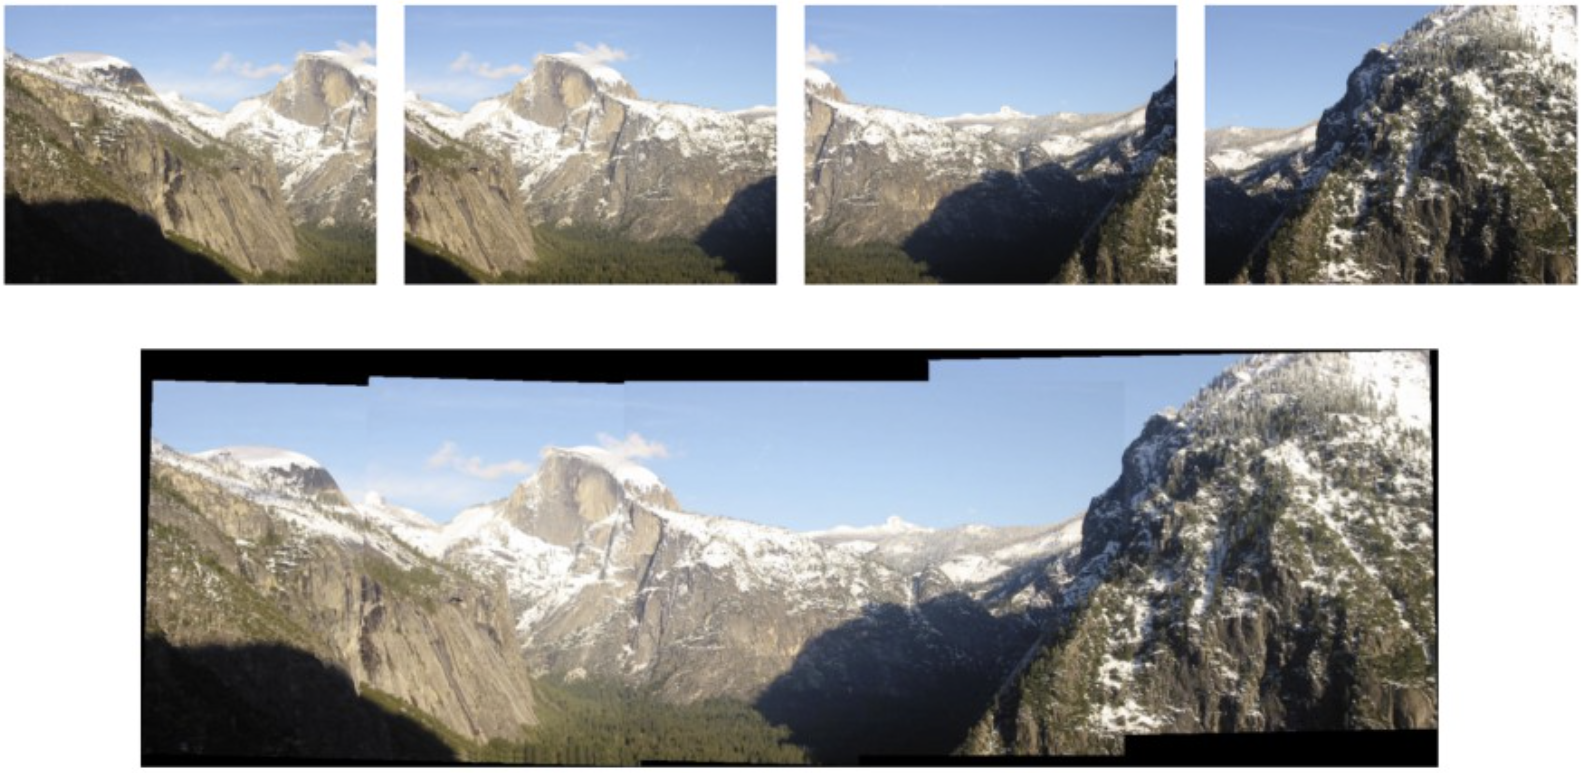
\includegraphics[width=1.0\textwidth]{stitching_1}
			\end{figure}
		\end{frame}


	\section{Computer vision}

		\begin{frame}
			\frametitle{Computer vision I}
			\begin{columns}
				\column{.4\textwidth}
					\begin{itemize}
		 		  	\item Verarbeitung und Analyse von Bildern
						\item Aufgaben
							\begin{itemize}
								\item Image denoising, image deblurring, ...
								\item Objekterkennung, Bildklassifikation, Segmentierung, ...
								\item ...
							\end{itemize}
					\end{itemize}
				\column{.4\textwidth}
					\begin{figure}[t]
						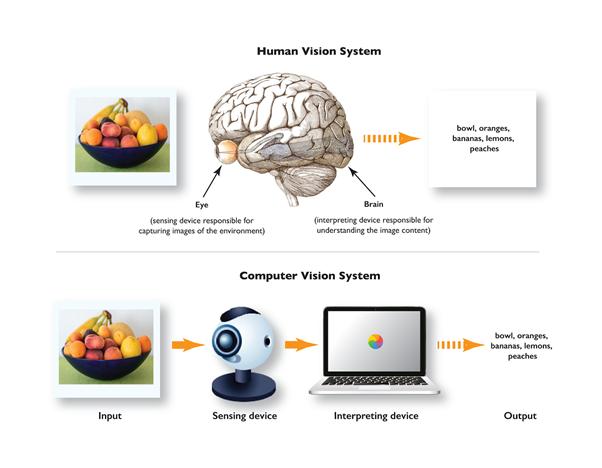
\includegraphics[width=1.5\textwidth]{computer_vision_2}
						\caption{\tiny Vision systems}
					\end{figure}
				\column{.1\textwidth}
			\end{columns}
		\end{frame}

		\begin{frame}
			\frametitle{Computer vision II}
			\begin{columns}
				\column{.4\textwidth}
			  	\begin{itemize}
						\item Anwendungsbereiche
							\begin{itemize}
								\vspace{\baselineskip}
								\item Medizin
								\item Automotive, Logistik
								\item Fotografie
								\item ...
							\end{itemize}

						\item Grundlagendisziplinen
							\begin{itemize}
								\item Mathematik und Statistik
								\item Computer science
								\item ...
							\end{itemize}
					\end{itemize}
				\column{.4\textwidth}
          \begin{figure}[t]
            
\includegraphics[width=1.0\textwidth]{computer_vision_1}
          \end{figure}
          \vspace{\baselineskip}
					\vspace{\baselineskip}
					\vspace{\baselineskip}
					\vspace{\baselineskip}
				\column{.1\textwidth}
			\end{columns}
			
		\end{frame}

  \section{Projektinhalte}

    \begin{frame}
      \frametitle{Projektinhalte}
			\begin{columns}
				\column{.5\textwidth}
		      \begin{itemize}
  		      \item Grundlagen der Bildverarbeitung
    		      \begin{itemize}
      		      \item Mathematisches Bildmodell
      	  	    \item Transformation von Bildern
          		  \item Merkmale von Bildern und Merkmalsextraktion
	          	  \item ...
	  	        \end{itemize}
  	  	    \item Programmierung
    	      	\begin{itemize}
	   		  	  \item Erste Schritte in Python und OpenCV
							\item Implementierung eines Algorithmus zum image stitching
    	    	\end{itemize}
		      \end{itemize}
				\column{.4\textwidth}
					\begin{figure}
						
\includegraphics[width=0.7\textwidth]{python_and_opencv}
					\end{figure}
			\end{columns}
    \end{frame}

  \section{Ziele des Projekts}

    \begin{frame}
      \frametitle{Ziele des Projekts}
      \begin{columns}
        \begin{column}{0.48\textwidth}
          \begin{figure}
            
\includegraphics[scale = 0.53]{images/projektziele.jpg}
          \end{figure}
        \end{column}
        \begin{column}{0.5\textwidth}
          \begin{itemize}
            \item Erlangen von mathematischen und technischen Grundkenntnissen der Bildverarbeitung
            \item Grundlegende Programmierkenntnisse in Python
            \item Python-Programm zum stitching von zwei oder mehreren Bildern
          \end{itemize}
        \end{column}
      \end{columns}
    \end{frame}

\end{document}
